%-------------------------------------------------------------------------------
\section{Overview}
%-------------------------------------------------------------------------------
\begin{figure*}[!th]
\begin{center}
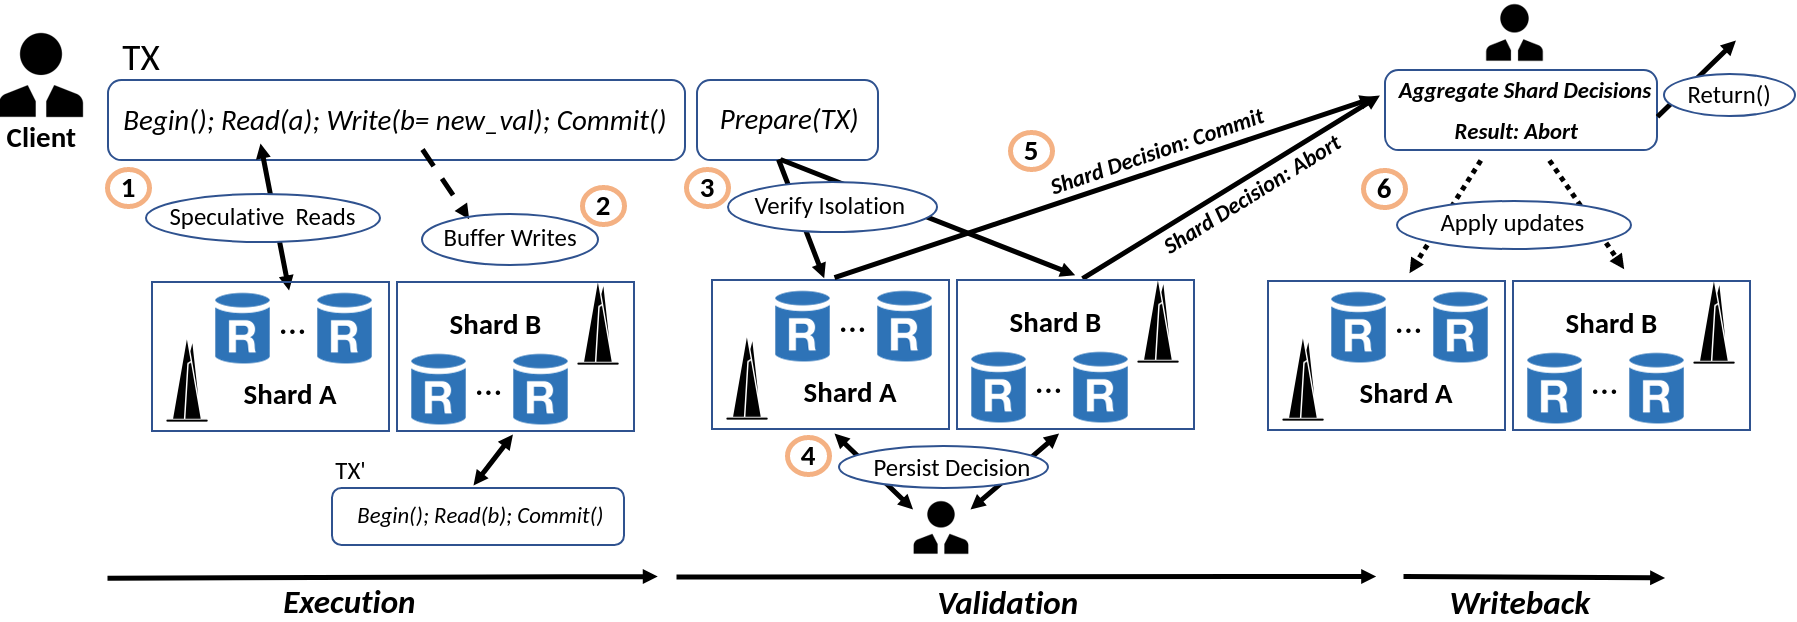
\includegraphics[width= \textwidth]{./figures/Archi.png}
\end{center}
\caption{{\em Transaction Lifecycle}. Clients execute remote reads (1) and buffer writes (2). For Committment, all involved shards verify isolation (3). If there are conflicting transactions (TX'), replicas in a shard (B) vote to Abort. A client persists a decision (4) that serves as Two-Phase-Commit Vote for each shard (5), and Commits a transaction if all shards vote to commit (6).}
\label{fig:Figure1}
\end{figure*}

\sys is designed to be scalable and leaderless and our architecture reflects this ethos. \sys{} is a sharded and replicated transactional key-value store.

\par \textbf{Transaction Execution} Transaction execution is driven by clients (removing costly all-to-all
communications amongst replicas) and consists of three phases. First, in an \textit{execution phase}, clients execute individual transactional operations. As is standard in optimistic
databases, reads are submitted to remote replicas while writes are buffered locally. \sys{} supports \textit{interactive} and cross-shard transactions: clients
can issue new operations based on the results of past operations to any shard in the system. \sys{} must additionally ensure that these read operations do not violate
Byzantine independence. In a second \textit{validation phase}, invidual shards in \sys{} must validate whether committing the transaction would violate serializability. For performance,
\sys{} allows invidiual replicas within to process requests out of order. \sys{} must additionally ensure that Byzantine actors cannot cause spurious aborts. Finally, \sys{} aggregates each shard decision in a \textit{commit phase} and determines the outcome of the transaction, notifying both the application and replicas in the system of the decision. Importantly, this decision must be preserved across failures, reconfigurations and Byzantine attacks. We describe each of these phases in turn in Section~\ref{}

\par \textbt{Transaction Recovery} To ensure progress, design a recovery mechanism that can finish stalled transactions. We describe this fallback mechanism in Section~\ref{}.

\nc{Florian's version in comments}
\sys is designed to be scalable and leaderless. Our architecture reflects this ethos. We briefly summarise it here before going into more detail in the later sections. 
In \sys, clients drive the entire transaction life cycle which can be broken down into three stages as shown in Figure \ref{fig:Figure1}: i) Execution, ii) Validation, and iii) Writeback. 
i) Clients \textit{speculatively execute} transactions themselves, invoking only remote read procedure calls (1) and buffering writes locally (2). Transactions may read and write arbitrarily and can span several data partitions (shards). Moreover, different clients may execute transactions concurrently, performing reads in different order at (a subset of) replicas within each shard. 
ii) Since execution is speculative, and clients are unaware of potential concurrency, they must \textit{validate} their transaction execution for Isolation correctness in order to be able to commit (3) \fs{This is the Prepare phase of 2PC. Every shard is one voter}. Intuitively, if there are no conflicting concurrent transactions, and a clients transaction observed a consistent snapshot of the database state then it may commit, and otherwise must retry or abort its transaction. Validation too, is client driven, and may happen in different order, both across different shards, as well as across replicas within each shard. For every relevant shard, a client must query potentially inconsistent replicas for their commitment vote, reconcile divergent votes into a single per-shard decision that maintains Isolation, and make this decision durable to avoid replay of contradictory decisions (4). 
iii) Lastly, a client aggregates all shard decisions (5) in atomic commit fashion and returns to the application. Asynchronously, it \textit{writes back} the decision to all involved replicas who apply the transaction to their local database state (6) \fs{This is the Commit phase of 2PC}.

Next, we outline the protocols for Execution, Validation and Writeback respectively. 

\iffalse
\fs{Old}
Indicus is a transactional database, offering clients the interface of interactive transactions with ACID guarantees. It is replicated for fault tolerance and can be sharded, in which case every shard is replicated. 

In Indicus, Clients are more than external participants who propose Transactions to be executed. Instead, Clients are first class citizens that rejoice in the fair treatment of democracy and take part in everyday system activities. Of course, such priviledge comes at the cost of added responsibilities. Concretely, Indicus does not provide a continuously and mysteriously operating black box Transaction machine, but implements a Quorum system, offering Clients the tools to operate the system itself. One the one hand, the simple paradigm of letting clients work for themselves is more scalable as replicas need to do less work and can service more clients. On the other hand, it naturally incentivises clients to be industrious, as they hold the keys to their own liveness. Clients that do not meet a certain standard for productivity may be excluded by the system; The joys of being permissioned.

Indicus follows a traditional optimistic concurrency control architecture as shown in Figure~\ref{fig:Figure1}. Clients speculatively execute their Transactions, issuing remote reads when necessary and buffering writes locally. As Clients execute their own Transactions they need not declare their read/write keys or values preemtively, but rather may conduct interactive Transactions, the most general Transaction model. Since execution is speculative and Clients are unaware of potential concurrency, they must validate their Transactions for Isolation correctness in order to be able to Commit. Intuitively, if there are no conflicting concurrent Transactions and a Client observed a consistent snapshot of the distributed Database state then it may commit, and otherwise it must abort or retry. Lastly, Transactions may span multiple shards, and hence the Commit/Abort decisions of each shard are aggregated in a Two Phase Commit manner in order to finalize a safety appropriate result. Most notably, in Indicus not just exeuction is Client driven but the entire Transaction life cycle, thus maximizing scalability and fairness while putting each Client in charge of its own liveness.
Next, we outline the protocols for Execution, Validation and Writeback respectively.

\fi
